%%%%%%%%%%%%%%%%%%%%%%%%%%%%%%%%%%%%%%%%%%%%%%%%%%%%%%%%%%%%%%%%%%%%%%%%%%%%%%%%%%%%%%%%%%%%%%%%%%%%%%%%%%%%%%%%%%%%%%%%%%%%%%%%%%%%%%%%%%%%%%%
%%%%%%%%%%%%%%%%%%%%%%%%%%%%%%%%%%%%%%%%%%%%%%%%%%%%%%%%%%%%%%%%%%%%%%%%%%%%%%%%%%%%%%%%%%%%%%%%%%%%%%%%%%%%%%%%%%%%%%%%%%%%%%%%%%%%%%%%%%%%%%%
\section{Hardware}
\label{sec:Hardware}
%%%%%%%%%%%%%%%%%%%%%%%%%%%%%%%%%%%%%%%%%%%%%%%%%%%%%%%%%%%%%%%%%%%%%%%%%%%%%%%%%%%%%%%%%%%%%%%%%%%%%%%%%%%%%%%%%%%%%%%%%%%%%%%%%%%%%%%%%%%%%%%
%%%%%%%%%%%%%%%%%%%%%%%%%%%%%%%%%%%%%%%%%%%%%%%%%%%%%%%%%%%%%%%%%%%%%%%%%%%%%%%%%%%%%%%%%%%%%%%%%%%%%%%%%%%%%%%%%%%%%%%%%%%%%%%%%%%%%%%%%%%%%%%

%%%%%%%%%%%%%%%%%%%%%%%%%%%%%%%%%%%%%%%%%%%%%%%%%%%%%%%%%%%%%%%%%%%%%%%%%%%%%%%%%%%%%%%%%%%%%%%%%%%%%%%%%%%%%%%%%%%%%%%%%%%%%%%%%%%%%%%%%%%%%%%
%%%%%%%%%%%%%%%%%%%%%%%%%%%%%%%%%%%%%%%%%%%%%%%%%%%%%%%%%%%%%%%%%%%%%%%%%%%%%%%%%%%%%%%%%%%%%%%%%%%%%%%%%%%%%%%%%%%%%%%%%%%%%%%%%%%%%%%%%%%%%%%
\begin{figure*}[th]
	
	\newsavebox{\faceDiagram}
	\sbox{\faceDiagram}	{
		\newcommand{\statcirc}[4]{
	\fill[opacity = 0.5, red,shift={(#1 cm,#2 cm)}, rotate=#3] (0,0) circle (#4); 
	\fill[opacity = 0.5, blue,shift={(#1 cm,#2 cm)},rotate=#3] (0,0) -- (180:#4) arc (180:0:#4) -- cycle;
	%	\draw[->,black,shift={(#1 cm,#2 cm)},rotate=#3] (#4, 0)
}

\newcommand{\drawArrow}[3]{
	\draw[->,>={Stealth[round]}, line width=0.75mm, black ,shift={(#1 cm,#2 cm)}, rotate=#3] (0,-0.5) -- (0,0.5); 
}

\newcommand{\drawchip}[3]{
	\tikzmath
	{
		\chipW = 0.35;
		\chipH = 0.4;
	}
	\fill[opacity = 0.75, darkgray, shift= {(#1 cm, #2 cm)}, rotate = #3, rounded corners] (-\chipH,-\chipW) rectangle (\chipH,\chipW);
	\fill[orange,shift= {(#1 cm, #2 cm)}, rotate = #3 ] (-0.25,0.2) circle (0.1);
}
\begin{tikzpicture}

	\tikzmath{
		\offsetAxis = 0.5;
		\offsetCent = 2.9;
		\diameter = 0.32;
	}
	\draw node (A) at (-0.5, 1.7) {};
	\draw node (B) at (0, 1.7) {};
	\drawchip{\offsetAxis}{\offsetCent}{0};
	\drawchip{-\offsetAxis}{-\offsetCent}{180};
	
	%Magnet North
	\statcirc{-\offsetAxis}{\offsetCent}{70}{\diameter};
	
	\drawArrow{-\offsetAxis}{\offsetCent}{70}
	
	%Magnet EAST
	\statcirc{\offsetCent}{\offsetAxis}{20}{\diameter};
	
	% Magnet West
	\statcirc{\offsetAxis}{-\offsetCent}{190}{\diameter};
	
	\statcirc{-\offsetCent}{-\offsetAxis}{45}{\diameter};
	
	\draw[gray, dashed] (-\offsetAxis,{\offsetCent + 1}) -- 
	(-\offsetAxis,{\offsetCent - 1});
	\draw[black,dotted] (0,0) circle (2.95);
	
	% 4 Cross Lines X
	\draw[black,dashed] (0,0) -- (4,0);
	\draw[black,dashed] (0,0) -- (-4,0);
	\draw[black,dashed] (0,0) -- (0,4);
	\draw[black,dashed] (0,0) -- (0,-4);
	
%	\draw[purple, dotted] ()
	% Dimensioned Variables
	\dimline[line style = {line width = 0.8, arrows = dimline reverse-dimline reverse}] {(A)}{(B)}{x};
	
	% Arc Radius
	\dimline[line style = {line width = 0.8}] {(0,0)} {++(150:2.95)}{R};
%	\dimline {(1,0)}{(-1,0)}{x};
\end{tikzpicture}
	}
	
	\newsavebox{\magnetDigitization}
	\sbox{\magnetDigitization}	{
		
\newcommand{\statcirc}[4]{
	\fill[red,shift={(#1 cm,#2 cm)}, rotate=#3] (0,0) circle (#4); 
	\fill[blue,shift={(#1 cm,#2 cm)},rotate=#3] (0,0) -- (180:#4) arc (180:0:#4) -- cycle;
	%	\draw[->,black,shift={(#1 cm,#2 cm)},rotate=#3] (#4, 0)
}

\newcommand{\drawArrow}[3]{
	\draw[->,>={Stealth[round]}, line width=0.75mm, black ,shift={(#1 cm,#2 cm)}, rotate=#3] (0,-1) -- (0,1); 
}

\begin{tikzpicture}[scale = 0.75]
\tikzmath{
	\offsetAxis = 0.5;
	\offsetCent = 2.9;
	\diameter = 0.75;
}

\foreach \i in {1,...,30}
{
	\draw[gray] (0,0) -- (\i * 12-6 : 2.8);
	\node[inner sep=0pt] at (-{\i * 12}+12: 3) {\i};
}
\node[circle,draw,inner sep=0pt, fill = green] at (-{18 * 12}+12: 3) {18};
\statcirc{0}{0}{-204-90}{\diameter};
\drawArrow{0}{0}{-204-90};
\draw[black,dashed] (0,0) -- (3,0);
\draw[black,dashed] (0,0) -- (-3,0);
\draw[black,dashed] (0,0) -- (0,3);
\draw[black,dashed] (0,0) -- (0,-3);
\draw[gray, dotted] (0,0) -- (-204: 3);
\draw[gray, dotted] (0,0) -- (-204: 3);
\draw [white, line width = 5pt] (2.1,0)  arc (0:360-204:2.1);
\draw [<->, >={Stealth[round]}] (2.1,0)  arc (0:360-204:2.1);
\node[circle,inner sep=3pt, fill = white]				at (90:2) {$\theta$};
\end{tikzpicture}
	}
	
	\newsavebox{\gridFigure}
	\sbox{\gridFigure}	{
		\begin{tikzpicture}[every node/.style={minimum size=2 cm-\pgflinewidth, outer sep=0pt}]
    \draw[step=2cm,color=black] (0,0) grid (4,4);

    \node[fill=orange] at (+1,+1) {};
   % \node[fill=yellow] at (+0.75,+0.75) {};
\end{tikzpicture}
	}
	%\begin{tikzpicture}[minimum width = 14 cm, minimum height = 6 cm]
	%\draw (0,0) -- (14,6);
	
	\begin{tikzpicture}[]
	%complexnode/.pic={\usebox{\mybox}}]
	
	\newcommand\xa{2};
	\newcommand\xb{2};
	\newcommand\ya{2};
	\newcommand\yb{2};
	
	\coordinate (smallNE) at (2,5);
	\coordinate (smallSE) at (2,5);
	\coordinate (smallSW) at (2,5);
	\coordinate (smallNW) at (2,5);
	
	\coordinate (bigNE) at (2,5);
	\coordinate (bigSE) at (2,5);
	\coordinate (bigSW) at (2,5);
	\coordinate (bigSE) at (2,5);
	
	\node[opacity = 0.95] at (3.15 cm, 2.85 cm) {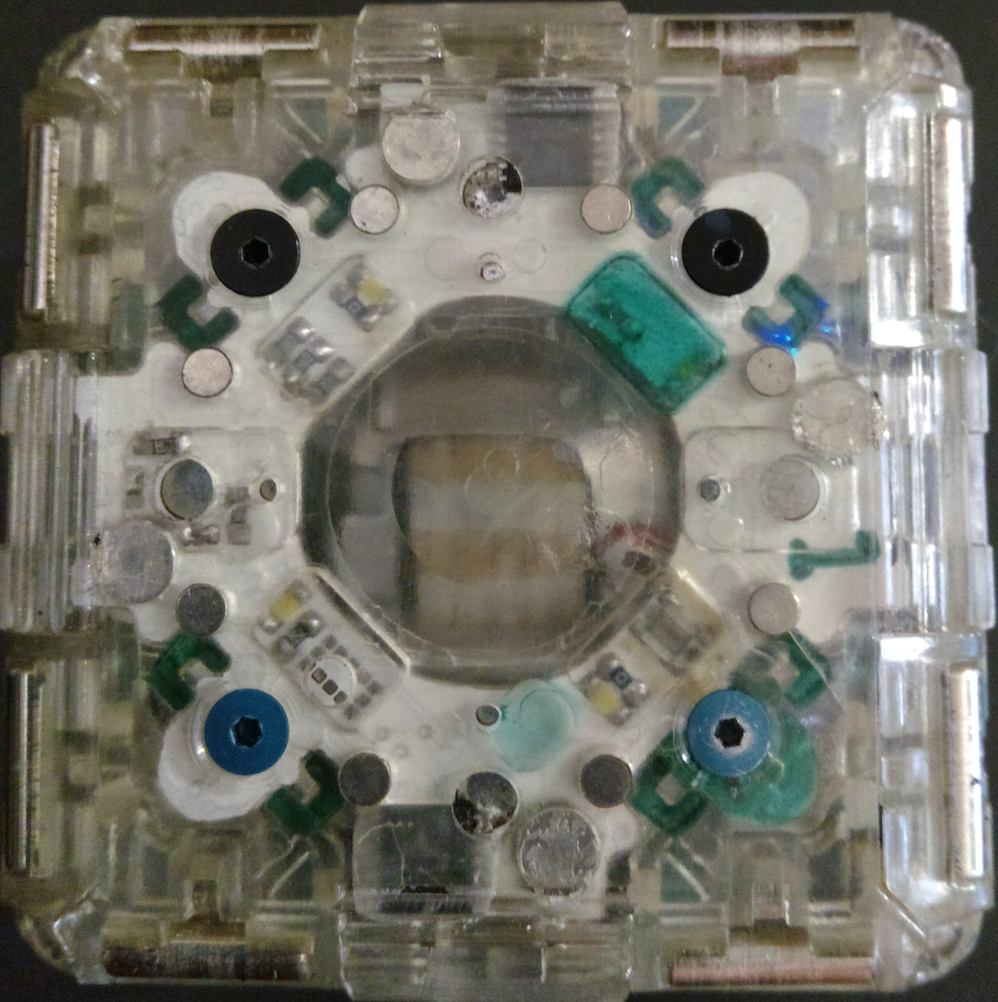
\includegraphics[width = 5.9 cm]{figures/face.png}};
	\node at (3 cm, 3 cm) {\usebox{\faceDiagram}};
	\node at (10 cm, 3 cm) {\usebox{\magnetDigitization}};
	\node at (15.5 cm, 2cm) {\usebox{\gridFigure}};
	
	%\node[fill=orange] at (3,3) {\textbf{18}};
	
	\tikzmath{
		\smallBoxX = 0.5;
		\smallBoxY = 2.9;
	}

	% Small Box around Magnet
	%\node[draw, purple, dotted, minimum size = 1.25 cm, rounded corners, thick] at (3.65cm , 7cm) {};
	
	\path[draw, purple, dotted, minimum size = 1.25 cm, rounded corners, ultra thick]
	(3*0.7, 6.25*0.7) --
	++(1.25, 0) --
	++(0, 1.25) --
	++(-1.25, 0) --
	cycle {};
	
	\node (a) at (12.5, 3){};
	\node (b) at (14.75, 3.4){};
	
	\draw[>={Stealth[round]}, purple,dashed, ultra thick, bend right, rounded corners = 1 cm, ->] (a) -- (13.75,5) -- (b);
	
	\draw[purple,dashed, thin] (2.7cm, 4.35cm + 1.25cm) -- ++(358: 4.8cm);
	\draw[purple,dashed, thin] (2.7cm, 4.35cm ) -- ++(323: 5.9cm);
	
	% Large Purple box
	\node[draw, purple, dotted, minimum size = 5 cm, rounded corners,ultra thick] at (10cm , 3cm) {};
	
	\node[] at (10cm , 0.2cm) {Discretizing Angle};
	%\draw (1,1) pic {complexnode} (4,4);
	
	\end{tikzpicture}
	
	
	
	
%	\newsavebox{\faceDiagram}
%	\sbox{\faceDiagram}	{
%		\newcommand{\statcirc}[4]{
	\fill[opacity = 0.5, red,shift={(#1 cm,#2 cm)}, rotate=#3] (0,0) circle (#4); 
	\fill[opacity = 0.5, blue,shift={(#1 cm,#2 cm)},rotate=#3] (0,0) -- (180:#4) arc (180:0:#4) -- cycle;
	%	\draw[->,black,shift={(#1 cm,#2 cm)},rotate=#3] (#4, 0)
}

\newcommand{\drawArrow}[3]{
	\draw[->,>={Stealth[round]}, line width=0.75mm, black ,shift={(#1 cm,#2 cm)}, rotate=#3] (0,-0.5) -- (0,0.5); 
}

\newcommand{\drawchip}[3]{
	\tikzmath
	{
		\chipW = 0.35;
		\chipH = 0.4;
	}
	\fill[opacity = 0.75, darkgray, shift= {(#1 cm, #2 cm)}, rotate = #3, rounded corners] (-\chipH,-\chipW) rectangle (\chipH,\chipW);
	\fill[orange,shift= {(#1 cm, #2 cm)}, rotate = #3 ] (-0.25,0.2) circle (0.1);
}
\begin{tikzpicture}

	\tikzmath{
		\offsetAxis = 0.5;
		\offsetCent = 2.9;
		\diameter = 0.32;
	}
	\draw node (A) at (-0.5, 1.7) {};
	\draw node (B) at (0, 1.7) {};
	\drawchip{\offsetAxis}{\offsetCent}{0};
	\drawchip{-\offsetAxis}{-\offsetCent}{180};
	
	%Magnet North
	\statcirc{-\offsetAxis}{\offsetCent}{70}{\diameter};
	
	\drawArrow{-\offsetAxis}{\offsetCent}{70}
	
	%Magnet EAST
	\statcirc{\offsetCent}{\offsetAxis}{20}{\diameter};
	
	% Magnet West
	\statcirc{\offsetAxis}{-\offsetCent}{190}{\diameter};
	
	\statcirc{-\offsetCent}{-\offsetAxis}{45}{\diameter};
	
	\draw[gray, dashed] (-\offsetAxis,{\offsetCent + 1}) -- 
	(-\offsetAxis,{\offsetCent - 1});
	\draw[black,dotted] (0,0) circle (2.95);
	
	% 4 Cross Lines X
	\draw[black,dashed] (0,0) -- (4,0);
	\draw[black,dashed] (0,0) -- (-4,0);
	\draw[black,dashed] (0,0) -- (0,4);
	\draw[black,dashed] (0,0) -- (0,-4);
	
%	\draw[purple, dotted] ()
	% Dimensioned Variables
	\dimline[line style = {line width = 0.8, arrows = dimline reverse-dimline reverse}] {(A)}{(B)}{x};
	
	% Arc Radius
	\dimline[line style = {line width = 0.8}] {(0,0)} {++(150:2.95)}{R};
%	\dimline {(1,0)}{(-1,0)}{x};
\end{tikzpicture}
%	}
%	
%	\newsavebox{\magnetDigitization}
%	\sbox{\magnetDigitization}	{
%		
\newcommand{\statcirc}[4]{
	\fill[red,shift={(#1 cm,#2 cm)}, rotate=#3] (0,0) circle (#4); 
	\fill[blue,shift={(#1 cm,#2 cm)},rotate=#3] (0,0) -- (180:#4) arc (180:0:#4) -- cycle;
	%	\draw[->,black,shift={(#1 cm,#2 cm)},rotate=#3] (#4, 0)
}

\newcommand{\drawArrow}[3]{
	\draw[->,>={Stealth[round]}, line width=0.75mm, black ,shift={(#1 cm,#2 cm)}, rotate=#3] (0,-1) -- (0,1); 
}

\begin{tikzpicture}[scale = 0.75]
\tikzmath{
	\offsetAxis = 0.5;
	\offsetCent = 2.9;
	\diameter = 0.75;
}

\foreach \i in {1,...,30}
{
	\draw[gray] (0,0) -- (\i * 12-6 : 2.8);
	\node[inner sep=0pt] at (-{\i * 12}+12: 3) {\i};
}
\node[circle,draw,inner sep=0pt, fill = green] at (-{18 * 12}+12: 3) {18};
\statcirc{0}{0}{-204-90}{\diameter};
\drawArrow{0}{0}{-204-90};
\draw[black,dashed] (0,0) -- (3,0);
\draw[black,dashed] (0,0) -- (-3,0);
\draw[black,dashed] (0,0) -- (0,3);
\draw[black,dashed] (0,0) -- (0,-3);
\draw[gray, dotted] (0,0) -- (-204: 3);
\draw[gray, dotted] (0,0) -- (-204: 3);
\draw [white, line width = 5pt] (2.1,0)  arc (0:360-204:2.1);
\draw [<->, >={Stealth[round]}] (2.1,0)  arc (0:360-204:2.1);
\node[circle,inner sep=3pt, fill = white]				at (90:2) {$\theta$};
\end{tikzpicture}
%	}
%	
%	\newsavebox{\gridFigure}
%	\sbox{\gridFigure}	{
%		\begin{tikzpicture}[every node/.style={minimum size=2 cm-\pgflinewidth, outer sep=0pt}]
    \draw[step=2cm,color=black] (0,0) grid (4,4);

    \node[fill=orange] at (+1,+1) {};
   % \node[fill=yellow] at (+0.75,+0.75) {};
\end{tikzpicture}
%	}
%	%\begin{tikzpicture}[minimum width = 14 cm, minimum height = 6 cm]
%	%\draw (0,0) -- (14,6);
%	
%	\begin{tikzpicture}[]
%	%complexnode/.pic={\usebox{\mybox}}]
%	
%	\newcommand\xa{2};
%	\newcommand\xb{2};
%	\newcommand\ya{2};
%	\newcommand\yb{2};
%	
%	\coordinate (smallNE) at (2,5);
%	\coordinate (smallSE) at (2,5);
%	\coordinate (smallSW) at (2,5);
%	\coordinate (smallNW) at (2,5);
%	
%	\coordinate (bigNE) at (2,5);
%	\coordinate (bigSE) at (2,5);
%	\coordinate (bigSW) at (2,5);
%	\coordinate (bigSE) at (2,5);
%	
%	\node[opacity = 0.95] at (4.25 cm, 4 cm) {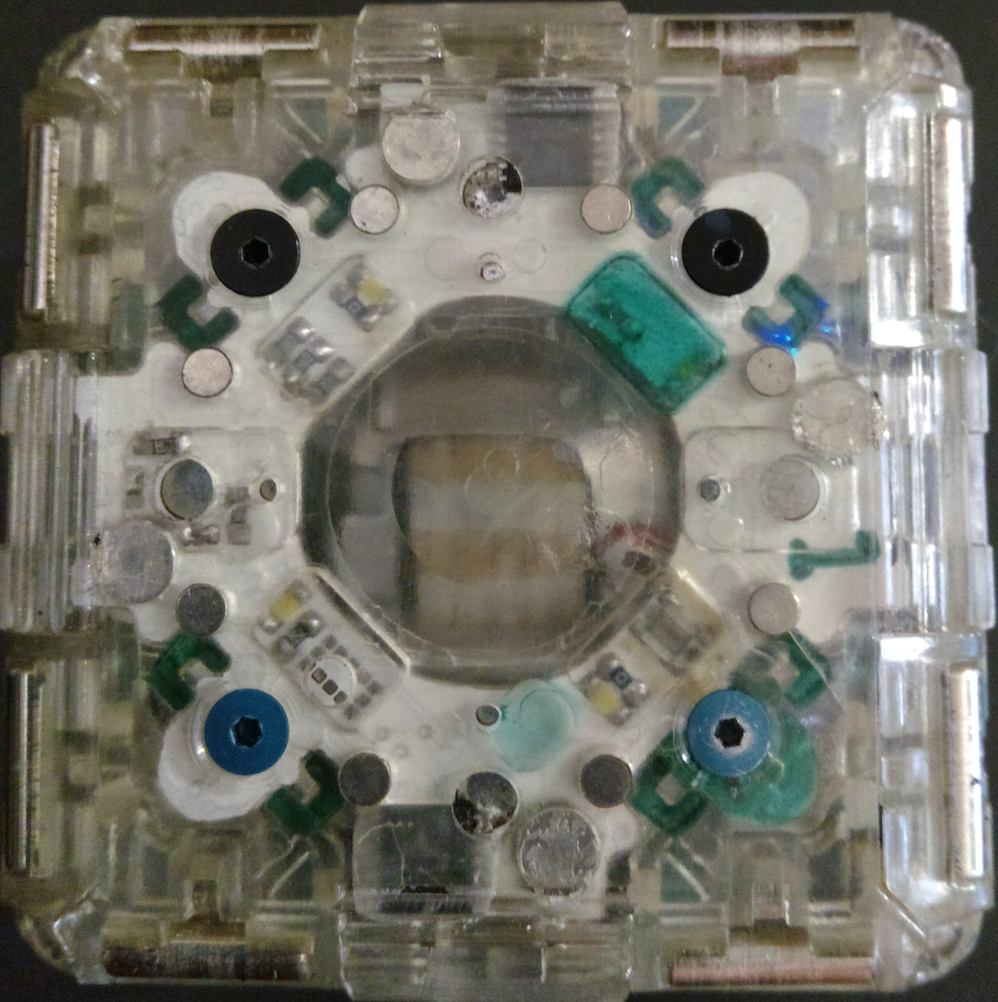
\includegraphics[width = 8 cm]{figures/face.png}};
%	\node at (4 cm, 4 cm) {\usebox{\faceDiagram}};
%	\node at (11 cm, 6 cm) {\usebox{\magnetDigitization}};
%	\node at (15 cm, 2cm) {\usebox{\gridFigure}};
%	
%	%\node[fill=orange] at (3,3) {\textbf{18}};
%	
%	\tikzmath{
%		\smallBoxX = 0.5;
%		\smallBoxY = 2.9;
%	}
%	
%	% Small Box around Magnet
%	%\node[draw, purple, dotted, minimum size = 1.25 cm, rounded corners, thick] at (3.65cm , 7cm) {};
%	
%	\path[draw, purple, dotted, minimum size = 1.25 cm, rounded corners, ultra thick]
%	(3, 6.25) --
%	++(1.25, 0) --
%	++(0, 1.25) --
%	++(-1.25, 0) --
%	cycle {};
%	
%	\node (a) at (13.5, 6){};
%	\node (b) at (15.75, 3.5){};
%	\draw[>={Stealth[round]}, purple,dashed, ultra thick, bend right, rounded corners = 1 cm, ->] (a) -- (15.75,6) -- (b);
%	\draw[purple,dashed, thin] (3.5cm, 6.25cm + 1.25cm) -- ++(10: 5cm);
%	\draw[purple,dashed, thin] (3.5cm, 6.25cm ) -- ++(332: 5.45cm);
%	
%	% Large Purple box
%	\node[draw, purple, dotted, minimum size = 4.8 cm, rounded corners,ultra thick] at (11cm , 6cm) {};
%	
%	%\draw (1,1) pic {complexnode} (4,4);
%	
%	\end{tikzpicture}
	
	\caption{Figure illustrating the \TagNamePlural. A tag consists of four permanent magnets placed according to two dimensions, (R) is the circle diameter, and x is the offset from the y axis. The right half of this figure shows a photo of one of the m-blocks superimposed with the magnets. The absolute angle of the magnet, relative to a line extending from the center of the face, is then digitized by an absolute magnetic encoder (black rectangle with orange dot) placed $x$ units to the right. }
	\label{fig:tagDiagram}
\end{figure*}
%%%%%%%%%%%%%%%%%%%%%%%%%%%%%%%%%%%%%%%%%%%%%%%%%%%%%%%%%%%%%%%%%%%%%%%%%%%%%%%%%%%%%%%%%%%%%%%%%%%%%%%%%%%%%%%%%%%%%%%%%%%%%%%%%%%%%%%%%%%%%%%
%%%%%%%%%%%%%%%%%%%%%%%%%%%%%%%%%%%%%%%%%%%%%%%%%%%%%%%%%%%%%%%%%%%%%%%%%%%%%%%%%%%%%%%%%%%%%%%%%%%%%%%%%%%%%%%%%%%%%%%%%%%%%%%%%%%%%%%%%%%%%%%
The ideal neighbor connectivity sensing solution would be inexpensive, robust and passive in order to help satisfy the ease of scalability in a modular robotics system where there may be hundreds or thousands of individual modules. It should also be precise, because individual errors in a repeated sequence of connections would be multiplicative and thus damaging to the concerted operation of a whole configuration of modules. In addition, it would not be enough to merely identify an object or even to detect which connecting faces are adjacent in the lattice or chain, because effective concerted motion between modules may require them to identify how they and their neighbors are oriented with respect to the larger configuration.

 Our new method for estimating the position of adjacent modules addresses both of these issues, and is illustrated with in Figure~\ref{fig:tagDiagram8}.  We introduce \tagNamePlural, arrangements of magnets mounted on the faces of modules.  The orientation of magnets which comprise \tagNamePlural can be measured by simple absolute magnetic encoder ICs, thereby reading information encoded in the orientation of the magnets.

%%%%%%%%%%%%%%%%%%%%%%%%%%%%%%%%%%%%%%%%%%%%%%%%%%%%%%%%%%%%%%%%%%%%%%%%%%%%%%%%%%%%%%%%%%%%%%%%%%%%%%%%%%%%%%%%%%%%%%%%%%%%%%%%%%%%%%%%%%%%%%%
%%%%%%%%%%%%%%%%%%%%%%%%%%%%%%%%%%%%%%%%%%%%%%%%%%%%%%%%%%%%%%%%%%%%%%%%%%%%%%%%%%%%%%%%%%%%%%%%%%%%%%%%%%%%%%%%%%%%%%%%%%%%%%%%%%%%%%%%%%%%%%%
\begin{table}[b]
	\caption{Information content in the \TagNamePlural encoding specification. The current system is limited due to practical considerations of the physical dimensions of the  PCBa's in the 3D M-Blocks, but will hopefully be extended into the future extension soon.}
	
	\begin{tabular}{ p{2cm}  p{1.5cm}  p{1.5cm}  p{1.5cm}}
		\hline
								& \textit{Current System} & Future Extension & Advanced Extended \\
		\hline
				\addlinespace[1ex]
		Magnets  				& 4 			 &	4				&	4	\\
		Digits 					& 30 			 &	24				&	48	\\
		No. Of Sensors 			& 2 			 &	4				&	4	\\
		\textit{Unique Tags} 	& \textbf{900} 	 & 331776			& 	~5,000,000\\
		
	\end{tabular}
	
	\label{tab:hardwareOverview}
\end{table}
%%%%%%%%%%%%%%%%%%%%%%%%%%%%%%%%%%%%%%%%%%%%%%%%%%%%%%%%%%%%%%%%%%%%%%%%%%%%%%%%%%%%%%%%%%%%%%%%%%%%%%%%%%%%%%%%%%%%%%%%%%%%%%%%%%%%%%%%%%%%%%%
%%%%%%%%%%%%%%%%%%%%%%%%%%%%%%%%%%%%%%%%%%%%%%%%%%%%%%%%%%%%%%%%%%%%%%%%%%%%%%%%%%%%%%%%%%%%%%%%%%%%%%%%%%%%%%%%%%%%%%%%%%%%%%%%%%%%%%%%%%%%%%%

The approach that \tagNamePlural~take towards this problem is a passive magnetic connector that uses a combination of dipole angles to communicate identity and relative rotational position. In this implementation, each face of each cube is encoded with a different combination of magnetic angles than every other face of every other cube. Magnetic rotary position sensors read these dipole angle combinations to determine which face is directly adjacent, and they identify the rotational angle of the face as well. All of this occurs using an un-powered array of magnets that provide static EM fields, readable at a hyperlocal distance.

The underlying hypothesis is that low cost and lack of RF transmission make magnets an attractive choice for a technology that may have to be implemented hundreds of times in a set of reconfigurable modules. The ability to use several such sensors at close proximity allows several to be used on each connecting face, providing enough data to read configuration as well as identity. The \tagNamePlural were designed and tested with the M-Blocks modular robots as the test bed, although nothing precludes their use in other circumstances.

%%%%%%%%%%%%%%%%%%%%%%%%%%%%%%%%%%%%%%%%%%%%%%%%%%%%%%%%%%%%%%%%%%%%%%%%%%%%%%%%%%%%%%%%%%%%%%%%%%%%%%%%%%%%%%%%%%%%%%%%%%%%%%%%%%%%%%%%%%%%%%%
%%%%%%%%%%%%%%%%%%%%%%%%%%%%%%%%%%%%%%%%%%%%%%%%%%%%%%%%%%%%%%%%%%%%%%%%%%%%%%%%%%%%%%%%%%%%%%%%%%%%%%%%%%%%%%%%%%%%%%%%%%%%%%%%%%%%%%%%%%%%%%%
\begin{table}[b]
  \caption{Basic info of the m-Blocks modular robots}

  \begin{tabular}{ p{3.4cm}  p{1.9cm} }
    \hline
    Actuation Directions & 6 \\
    Mass  & 150\,g \\
    Characterist Dimension & 50\,mm \\dra
    Total Parts  & 216 \\
    Actuated Moving Parts  & 10 \\
    Est. Cost & \$130 \\

  \end{tabular}

    \label{tab:hardwareOverviewTable}
\end{table}
%%%%%%%%%%%%%%%%%%%%%%%%%%%%%%%%%%%%%%%%%%%%%%%%%%%%%%%%%%%%%%%%%%%%%%%%%%%%%%%%%%%%%%%%%%%%%%%%%%%%%%%%%%%%%%%%%%%%%%%%%%%%%%%%%%%%%%%%%%%%%%%
%%%%%%%%%%%%%%%%%%%%%%%%%%%%%%%%%%%%%%%%%%%%%%%%%%%%%%%%%%%%%%%%%%%%%%%%%%%%%%%%%%%%%%%%%%%%%%%%%%%%%%%%%%%%%%%%%%%%%%%%%%%%%%%%%%%%%%%%%%%%%%%

The \tagNamePlural are implemented using absolute magnetic encoders from Austrian Micro Systems. Each active module has been outfitted with a circuit board that
includes two AS5048B absolute magnetic encoders, a light sensor, and several LEDs. The circuit boards are driven from the central processor 
through an I2C I/O expander.

%%%%%%%%%%%%%%%%%%%%%%%%%%%%%%%%%%%%%%%%%%%%%%%%%%%%%%%%%%%%%%%%%%%%%%%%%%%%%%%%%%%%%%%%%%%%%%%%%%%%%%%%%%%%%%%%%%%%%%%%%%%%%%%%%%%%%%%%%%%%%%%
%%%%%%%%%%%%%%%%%%%%%%%%%%%%%%%%%%%%%%%%%%%%%%%%%%%%%%%%%%%%%%%%%%%%%%%%%%%%%%%%%%%%%%%%%%%%%%%%%%%%%%%%%%%%%%%%%%%%%%%%%%%%%%%%%%%%%%%%%%%%%%%
\subsection{\tagNamePlural Characterization}
\label{sec:tagsCharacterize}
%%%%%%%%%%%%%%%%%%%%%%%%%%%%%%%%%%%%%%%%%%%%%%%%%%%%%%%%%%%%%%%%%%%%%%%%%%%%%%%%%%%%%%%%%%%%%%%%%%%%%%%%%%%%%%%%%%%%%%%%%%%%%%%%%%%%%%%%%%%%%%%
%%%%%%%%%%%%%%%%%%%%%%%%%%%%%%%%%%%%%%%%%%%%%%%%%%%%%%%%%%%%%%%%%%%%%%%%%%%%%%%%%%%%%%%%%%%%%%%%%%%%%%%%%%%%%%%%%%%%%%%%%%%%%%%%%%%%%%%%%%%%%%%

While the exact performance of the \tagName system that will be be implementation Dependant i.e. different size/shape magnets, encoder ICs, etc... we performed two categories of experimentation to demonstrate that our implementation of the \tagName concept is feasible and useful in the context of modular robots. The first section~\ref{sec:characterize} attempts to characterize the \tagNamePlural in terms of repeatability and accuracy of multiple measurements under varying conditions and to investigate the behavior when tags are misaligned. 

While the angular resolution of the magnetic angular encoders that we used is very high, 14 bits for the ams5048b used in this work, these readings are only repeatable under ideal conditions. There are many factors which influence the accuracy of readings of the sensors in the context of the \tagNamePlural. We have identified the following factors 1. Alignment of the magnetic sensor relative to the face of the module, 2. relative alignment of the face containing the tag to the face containing the reader. 3. variability of the magnetic field direction in the manufacture of the magnets. 4. Mechanical alignment of the magnets in reference to the tag. 5. Effects of external magnetic fields.

While factors 1 and 4, (mechanical alignment of magnets and sensors) are appear to be a significant factor in our implementation due to the hand-assembly nature of the prototype system, these should be less of a concern in large scale systems which are properly manufactured.

\begin{figure}[h]
	% Data

\begin{tikzpicture}
\begin{axis}[
height=4cm,
width=9cm,
%            ybar interval,      % <-- this causes the `xticks' to be centered
ymin= 0, ymax=5,
xmin=-11, xmax=11,
grid=both,
minor y tick num=1,
%yminorgrids=true,
tick align=outside, % <-- this positions the ticks "outside"
]
\addplot+ [
ybar interval,
mark=none,
fill=blue!25,   % fill the bars again
] coordinates {

	(-10,0)	%
	(-9,0)	%
	(-8,0)	%
	(-7,1)	%
	(-6,0)	%1
	(-5,1)	%11
	(-4,1)	%11
	(-3,1)	%111111
	(-2,2)	%11111
	(-1,3)	%111111
	 (0,4)	%11111
	 (1,3)	%1
	 (2,5)	%
	 (3,4)	%
	 (4,3)	%
	 (5,1)	%
	 (6,1)	%
	 (7,1)	%
	 (8,0)	%
	 (9,0)	%
	 (10,1)	%

};

\addplot+ [
ybar interval,
mark=none,
fill=black,   % fill the bars again
] coordinates {
	(-6.05,16) 
	(-5.95,16) 
};

\addplot+ [
ybar interval,
mark=none,
fill=black,   % fill the bars again
] coordinates {
	(6.05,16) 
	(5.95,16) 
};
\end{axis}

\end{tikzpicture}
	\caption{Histogram of one sensor face reading the same tag multiple times. The Boundary lines represents tags that will not be read correctly.}
	\label{fig:histogram}
\end{figure}


%%%%%%%%%%%%%%%%%%%%%%%%%%%%%%%%%%%%%%%%%%%%%%%%%%%%%%%%%%%%%%%%%%%%%%%%%%%%%%%%%%%%%%%%%%%%%%%%%%%%%%%%%%%%%%%%%%%%%%%%%%%%%%%%%%%%%%%%%%%%%%
%%%%%%%%%%%%%%%%%%%%%%%%%%%%%%%%%%%%%%%%%%%%%%%%%%%%%%%%%%%%%%%%%%%%%%%%%%%%%%%%%%%%%%%%%%%%%%%%%%%%%%%%%%%%%%%%%%%%%%%%%%%%%%%%%%%%%%%%%%%%%%
\begin{figure}[h]
	\begin{tikzpicture}
\begin{axis}[view={-20}{20}, grid=both]
\addplot3[surf] file {data.txt};
\end{axis}
\end{tikzpicture}
       
	\caption{Figure showing the error in the reading from a reader reading a tag as it is moved in X and Y relative to perfect alignment.}
	\label{fig:histogram}
\end{figure}
%%%%%%%%%%%%%%%%%%%%%%%%%%%%%%%%%%%%%%%%%%%%%%%%%%%%%%%%%%%%%%%%%%%%%%%%%%%%%%%%%%%%%%%%%%%%%%%%%%%%%%%%%%%%%%%%%%%%%%%%%%%%%%%%%%%%%%%%%%%%%%
%%%%%%%%%%%%%%%%%%%%%%%%%%%%%%%%%%%%%%%%%%%%%%%%%%%%%%%%%%%%%%%%%%%%%%%%%%%%%%%%%%%%%%%%%%%%%%%%%%%%%%%%%%%%%%%%%%%%%%%%%%%%%%%%%%%%%%%%%%%%%%